\documentclass{standalone}
\usepackage{tikz}
\usetikzlibrary{patterns, positioning}
\usepackage[sfdefault]{ClearSans} %% option 'sfdefault' activates Clear Sans as the default text font
\usepackage[T1]{fontenc}

\begin{document}
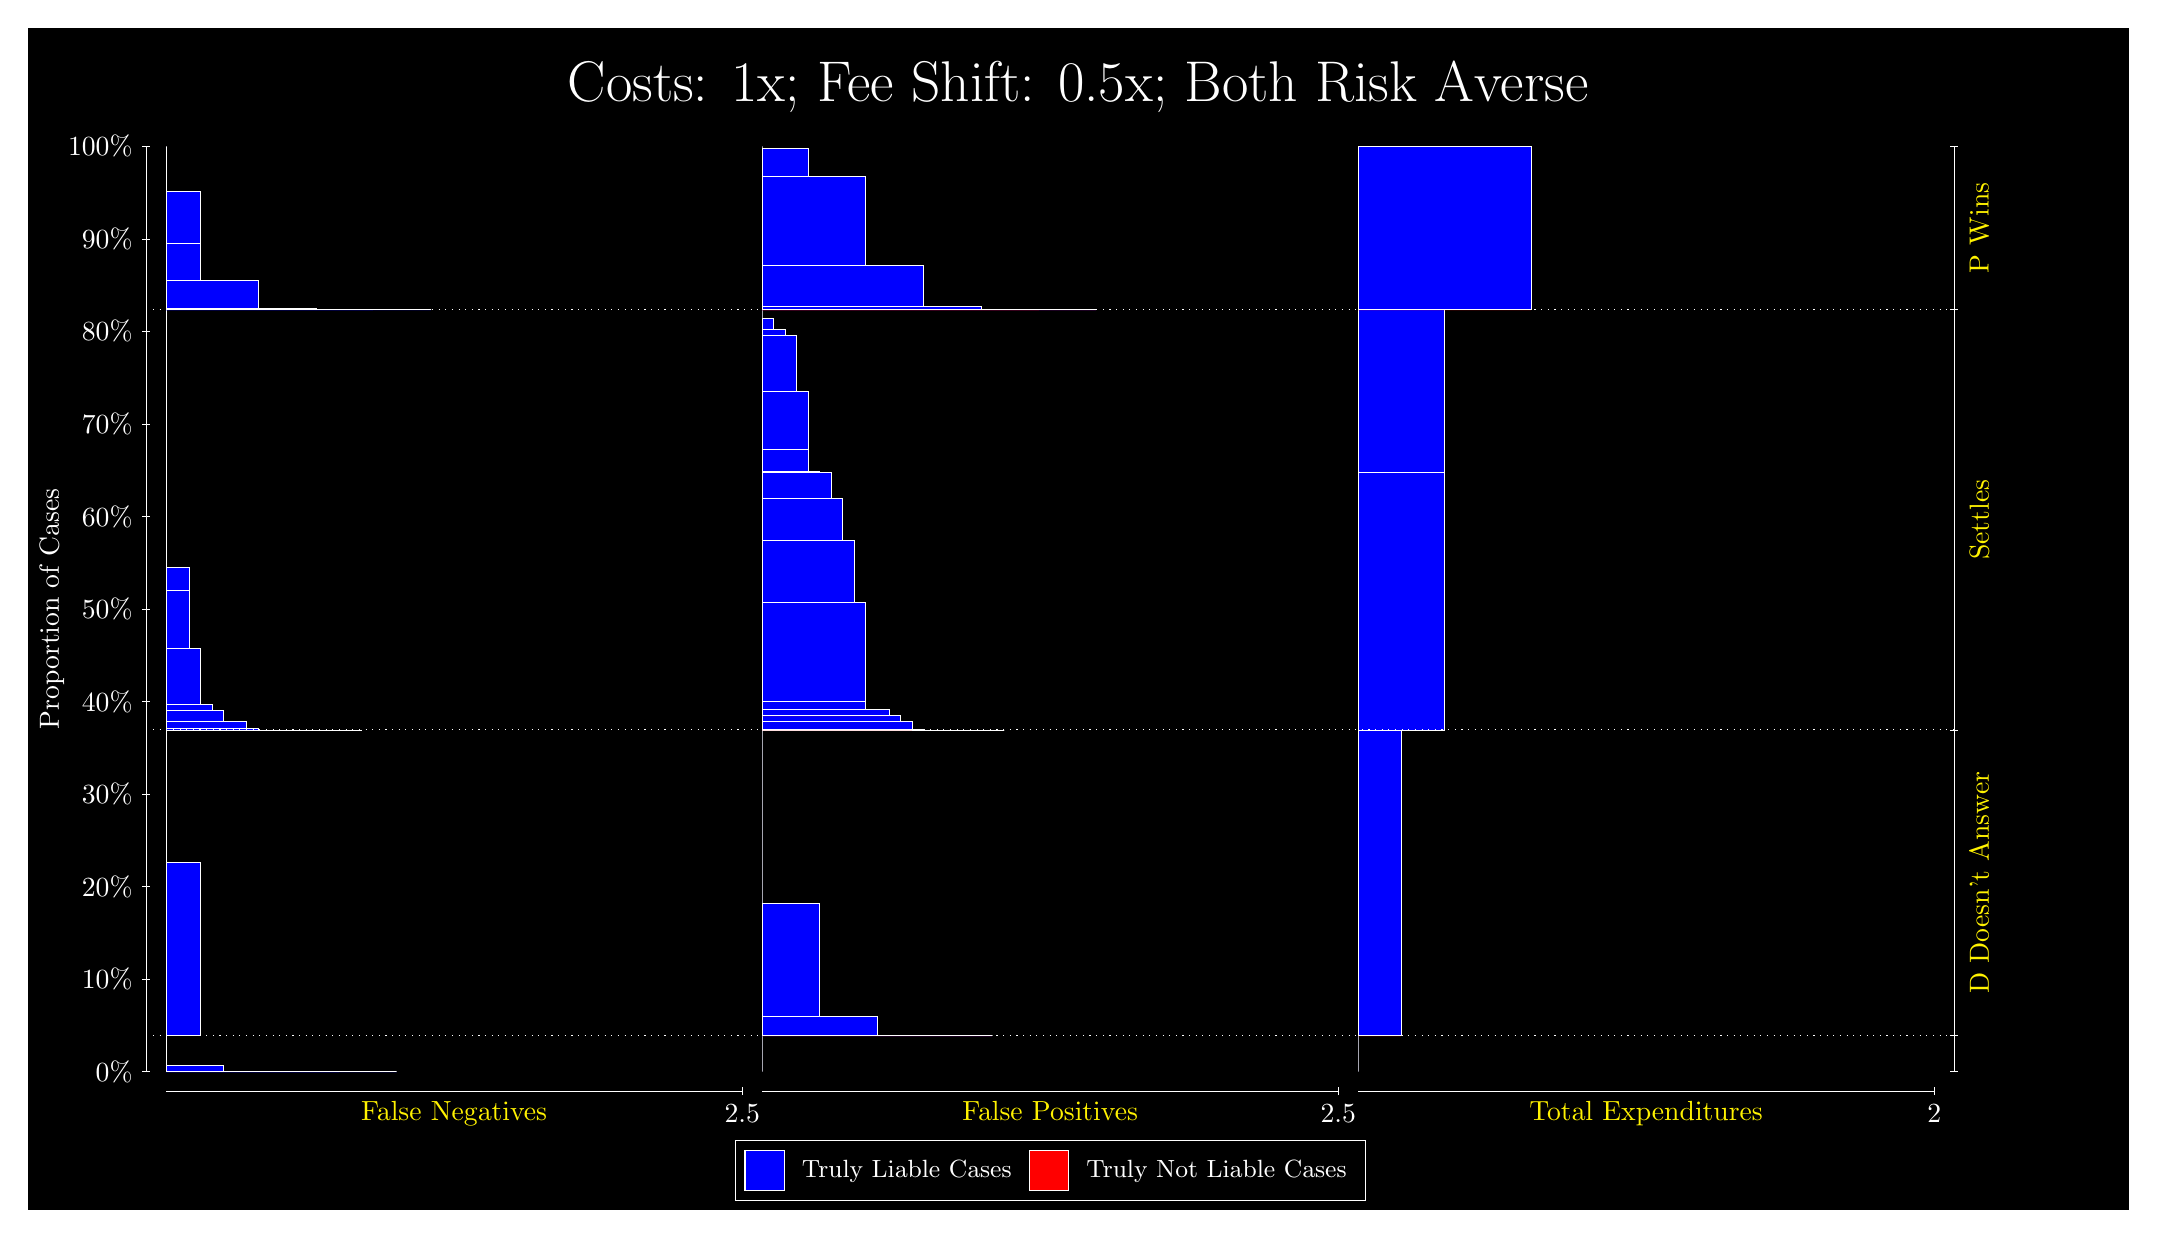
\begin{tikzpicture}
\draw[fill=black] (0,0) rectangle (26.667,15);
\draw[text=white] (0,13.5) rectangle (26.667,15) node[midway] {\huge Costs: 1x; Fee Shift: 0.5x; Both Risk Averse};
\draw[white, very thin] (1.5,1.75) -- (1.5,13.5);
\node[rotate=90, text=white, anchor=center] at (0.3, 7.625) {Proportion of Cases};
\draw[white, very thin] (1.45,1.75) -- (1.55,1.75);
\node[text=white, anchor=east] at (1.45, 1.75) {0\%};
\draw[white, very thin] (1.45,2.925) -- (1.55,2.925);
\node[text=white, anchor=east] at (1.45, 2.925) {10\%};
\draw[white, very thin] (1.45,4.1) -- (1.55,4.1);
\node[text=white, anchor=east] at (1.45, 4.1) {20\%};
\draw[white, very thin] (1.45,5.275) -- (1.55,5.275);
\node[text=white, anchor=east] at (1.45, 5.275) {30\%};
\draw[white, very thin] (1.45,6.45) -- (1.55,6.45);
\node[text=white, anchor=east] at (1.45, 6.45) {40\%};
\draw[white, very thin] (1.45,7.625) -- (1.55,7.625);
\node[text=white, anchor=east] at (1.45, 7.625) {50\%};
\draw[white, very thin] (1.45,8.8) -- (1.55,8.8);
\node[text=white, anchor=east] at (1.45, 8.8) {60\%};
\draw[white, very thin] (1.45,9.975) -- (1.55,9.975);
\node[text=white, anchor=east] at (1.45, 9.975) {70\%};
\draw[white, very thin] (1.45,11.15) -- (1.55,11.15);
\node[text=white, anchor=east] at (1.45, 11.15) {80\%};
\draw[white, very thin] (1.45,12.325) -- (1.55,12.325);
\node[text=white, anchor=east] at (1.45, 12.325) {90\%};
\draw[white, very thin] (1.45,13.5) -- (1.55,13.5);
\node[text=white, anchor=east] at (1.45, 13.5) {100\%};

\draw[white, very thin] (24.457,1.75) -- (24.457,13.5);
\draw[white, very thin] (24.407,1.75) -- (24.507,1.75);
\node[anchor=west] at (24.407, 1.75) {};
\draw[white, very thin] (24.407,2.206) -- (24.507,2.206);
\node[anchor=west] at (24.407, 2.206) {};
\draw[white, very thin] (24.407,6.0896) -- (24.507,6.0896);
\node[anchor=west] at (24.407, 6.0896) {};
\draw[white, very thin] (24.407,11.427) -- (24.507,11.427);
\node[anchor=west] at (24.407, 11.427) {};
\draw[white, very thin] (24.407,13.5) -- (24.507,13.5);
\node[anchor=west] at (24.407, 13.5) {};

\draw[white, very thin, fill=blue] (1.75,1.75) rectangle (4.6775,1.75);
\draw[white, very thin, fill=blue] (1.75,1.75) rectangle (3.9457,1.75);
\draw[white, very thin, fill=blue] (1.75,1.75) rectangle (3.2138,1.7506);
\draw[white, very thin, fill=blue] (1.75,1.7506) rectangle (2.4819,1.8247);
\draw[white, very thin, fill=red] (1.75,1.8247) rectangle (1.75,1.8247);
\draw[white, very thin, fill=blue] (1.75,1.8247) rectangle (1.75,2.206);
\draw[white, very thin, fill=blue] (1.75,2.206) rectangle (2.1891,4.4041);
\draw[white, very thin, fill=red] (1.75,4.4041) rectangle (1.75,4.4041);
\draw[white, very thin, fill=blue] (1.75,4.4041) rectangle (1.75,6.0896);
\draw[white, very thin, fill=blue] (1.75,6.0896) rectangle (4.2384,6.0896);
\draw[white, very thin, fill=blue] (1.75,6.0896) rectangle (3.9457,6.0896);
\draw[white, very thin, fill=blue] (1.75,6.0896) rectangle (3.6529,6.0896);
\draw[white, very thin, fill=blue] (1.75,6.0896) rectangle (3.5065,6.0897);
\draw[white, very thin, fill=blue] (1.75,6.0897) rectangle (3.3602,6.0897);
\draw[white, very thin, fill=blue] (1.75,6.0897) rectangle (3.2138,6.0897);
\draw[white, very thin, fill=blue] (1.75,6.0897) rectangle (3.0674,6.0899);
\draw[white, very thin, fill=blue] (1.75,6.0899) rectangle (2.921,6.1137);
\draw[white, very thin, fill=blue] (1.75,6.1137) rectangle (2.7746,6.2031);
\draw[white, very thin, fill=blue] (1.75,6.2031) rectangle (2.6283,6.2035);
\draw[white, very thin, fill=blue] (1.75,6.2035) rectangle (2.4819,6.3373);
\draw[white, very thin, fill=blue] (1.75,6.3373) rectangle (2.3355,6.414);
\draw[white, very thin, fill=blue] (1.75,6.414) rectangle (2.1891,7.1287);
\draw[white, very thin, fill=blue] (1.75,7.1287) rectangle (2.0428,7.8677);
\draw[white, very thin, fill=blue] (1.75,7.8677) rectangle (2.0428,8.1484);
\draw[white, very thin, fill=blue] (1.75,8.1484) rectangle (1.8964,8.1583);
\draw[white, very thin, fill=red] (1.75,8.1583) rectangle (1.75,8.1583);
\draw[white, very thin, fill=blue] (1.75,8.1583) rectangle (1.75,11.427);
\draw[white, very thin, fill=blue] (1.75,11.427) rectangle (5.1167,11.427);
\draw[white, very thin, fill=blue] (1.75,11.427) rectangle (4.3848,11.427);
\draw[white, very thin, fill=blue] (1.75,11.427) rectangle (3.6529,11.448);
\draw[white, very thin, fill=blue] (1.75,11.448) rectangle (2.921,11.805);
\draw[white, very thin, fill=blue] (1.75,11.805) rectangle (2.1891,12.265);
\draw[white, very thin, fill=blue] (1.75,12.265) rectangle (2.1891,12.933);
\draw[white, very thin, fill=red] (1.75,12.933) rectangle (1.75,12.933);
\draw[white, very thin, fill=blue] (1.75,12.933) rectangle (1.75,13.5);
\draw[white, very thin, fill=red] (9.3189,1.75) rectangle (9.3189,1.75);
\draw[white, very thin, fill=blue] (9.3189,1.75) rectangle (9.3189,2.206);
\draw[white, very thin, fill=red] (9.3189,2.206) rectangle (12.246,2.206);
\draw[white, very thin, fill=blue] (9.3189,2.206) rectangle (12.246,2.206);
\draw[white, very thin, fill=blue] (9.3189,2.206) rectangle (11.515,2.2081);
\draw[white, very thin, fill=blue] (9.3189,2.2081) rectangle (10.783,2.4564);
\draw[white, very thin, fill=blue] (9.3189,2.4564) rectangle (10.051,3.8916);
\draw[white, very thin, fill=blue] (9.3189,3.8916) rectangle (9.3189,6.0896);
\draw[white, very thin, fill=red] (9.3189,6.0896) rectangle (12.393,6.0896);
\draw[white, very thin, fill=blue] (9.3189,6.0896) rectangle (12.393,6.0896);
\draw[white, very thin, fill=red] (9.3189,6.0896) rectangle (12.1,6.0896);
\draw[white, very thin, fill=blue] (9.3189,6.0896) rectangle (12.1,6.0896);
\draw[white, very thin, fill=red] (9.3189,6.0896) rectangle (11.807,6.0896);
\draw[white, very thin, fill=blue] (9.3189,6.0896) rectangle (11.807,6.0898);
\draw[white, very thin, fill=blue] (9.3189,6.0898) rectangle (11.661,6.0898);
\draw[white, very thin, fill=red] (9.3189,6.0898) rectangle (11.515,6.0898);
\draw[white, very thin, fill=blue] (9.3189,6.0898) rectangle (11.515,6.0898);
\draw[white, very thin, fill=blue] (9.3189,6.0898) rectangle (11.368,6.0903);
\draw[white, very thin, fill=red] (9.3189,6.0903) rectangle (11.222,6.0903);
\draw[white, very thin, fill=blue] (9.3189,6.0903) rectangle (11.222,6.1964);
\draw[white, very thin, fill=blue] (9.3189,6.1964) rectangle (11.075,6.2704);
\draw[white, very thin, fill=red] (9.3189,6.2704) rectangle (10.929,6.2704);
\draw[white, very thin, fill=blue] (9.3189,6.2704) rectangle (10.929,6.3518);
\draw[white, very thin, fill=blue] (9.3189,6.3518) rectangle (10.783,6.3523);
\draw[white, very thin, fill=blue] (9.3189,6.3523) rectangle (10.636,6.4574);
\draw[white, very thin, fill=red] (9.3189,6.4574) rectangle (10.636,6.4574);
\draw[white, very thin, fill=blue] (9.3189,6.4574) rectangle (10.636,7.7046);
\draw[white, very thin, fill=blue] (9.3189,7.7046) rectangle (10.49,8.4942);
\draw[white, very thin, fill=blue] (9.3189,8.4942) rectangle (10.344,9.036);
\draw[white, very thin, fill=blue] (9.3189,9.036) rectangle (10.197,9.3587);
\draw[white, very thin, fill=blue] (9.3189,9.3587) rectangle (10.051,9.3686);
\draw[white, very thin, fill=blue] (9.3189,9.3686) rectangle (9.9044,9.6493);
\draw[white, very thin, fill=blue] (9.3189,9.6493) rectangle (9.9044,10.388);
\draw[white, very thin, fill=blue] (9.3189,10.388) rectangle (9.758,11.103);
\draw[white, very thin, fill=blue] (9.3189,11.103) rectangle (9.6116,11.18);
\draw[white, very thin, fill=blue] (9.3189,11.18) rectangle (9.4652,11.314);
\draw[white, very thin, fill=blue] (9.3189,11.314) rectangle (9.3189,11.427);
\draw[white, very thin, fill=red] (9.3189,11.427) rectangle (13.564,11.427);
\draw[white, very thin, fill=blue] (9.3189,11.427) rectangle (13.564,11.427);
\draw[white, very thin, fill=red] (9.3189,11.427) rectangle (12.832,11.427);
\draw[white, very thin, fill=blue] (9.3189,11.427) rectangle (12.832,11.428);
\draw[white, very thin, fill=red] (9.3189,11.428) rectangle (12.1,11.428);
\draw[white, very thin, fill=blue] (9.3189,11.428) rectangle (12.1,11.472);
\draw[white, very thin, fill=red] (9.3189,11.472) rectangle (11.368,11.472);
\draw[white, very thin, fill=blue] (9.3189,11.472) rectangle (11.368,11.995);
\draw[white, very thin, fill=red] (9.3189,11.995) rectangle (10.636,11.995);
\draw[white, very thin, fill=blue] (9.3189,11.995) rectangle (10.636,13.123);
\draw[white, very thin, fill=blue] (9.3189,13.123) rectangle (9.9044,13.479);
\draw[white, very thin, fill=blue] (9.3189,13.479) rectangle (9.3189,13.5);
\draw[white, very thin, fill=red] (16.888,1.75) rectangle (16.888,1.75);
\draw[white, very thin, fill=blue] (16.888,1.75) rectangle (16.888,2.206);
\draw[white, very thin, fill=red] (16.888,2.206) rectangle (17.437,2.206);
\draw[white, very thin, fill=blue] (16.888,2.206) rectangle (17.437,6.0896);
\draw[white, very thin, fill=red] (16.888,6.0896) rectangle (17.986,6.0896);
\draw[white, very thin, fill=blue] (16.888,6.0896) rectangle (17.986,9.3665);
\draw[white, very thin, fill=red] (16.888,9.3665) rectangle (17.986,9.3665);
\draw[white, very thin, fill=blue] (16.888,9.3665) rectangle (17.986,11.427);
\draw[white, very thin, fill=red] (16.888,11.427) rectangle (19.083,11.427);
\draw[white, very thin, fill=blue] (16.888,11.427) rectangle (19.083,13.5);
\draw[white, dotted] (1.5,2.206) -- (24.457,2.206);
\draw[white, dotted] (1.5,6.0896) -- (24.457,6.0896);
\draw[white, dotted] (1.5,11.427) -- (24.457,11.427);
\draw[white, very thin] (1.75,1.5) -- (9.0689,1.5);
\node[text=yellow, anchor=north] at (5.4094, 1.5) {False Negatives};
\draw[white, very thin] (9.0689,1.45) -- (9.0689,1.55);
\node[text=white, anchor=north] at (9.0689, 1.45) {2.5};

\draw[white, very thin] (9.3189,1.5) -- (16.638,1.5);
\node[text=yellow, anchor=north] at (12.978, 1.5) {False Positives};
\draw[white, very thin] (16.638,1.45) -- (16.638,1.55);
\node[text=white, anchor=north] at (16.638, 1.45) {2.5};

\draw[white, very thin] (16.888,1.5) -- (24.207,1.5);
\node[text=yellow, anchor=north] at (20.547, 1.5) {Total Expenditures};
\draw[white, very thin] (24.207,1.45) -- (24.207,1.55);
\node[text=white, anchor=north] at (24.207, 1.45) {2};


\node[text=yellow, centered, rotate=90] at (24.777, 4.1478) {D Doesn't Answer};
\node[text=yellow, centered, rotate=90] at (24.777, 8.7585) {Settles};
\node[text=yellow, centered, rotate=90] at (24.777, 12.464) {P Wins};

\draw (12.978300999999998,1.5) node[draw=none] (baseCoordinate) {};
\begin{scope}[align=center]
        \matrix[scale=0.5, draw=white, below=0.5cm of baseCoordinate, nodes={draw}, column sep=0.1cm]{
            \node[rectangle, draw, minimum width=0.5cm, minimum height=0.5cm, fill=blue] {}; &
            \node[draw=none, font=\small, text=white] (B) {Truly Liable Cases}; &
            \node[rectangle, draw, minimum width=0.5cm, minimum height=0.5cm, fill=red] {}; &
            \node[draw=none, font=\small, text=white] (B) {Truly Not Liable Cases}; \\
            };
\end{scope}

\end{tikzpicture}
\end{document}